\documentclass[paper-main.tex]{subfiles}


\begin{document}


% Optical microphone
% aim of optical microphone: play back injected sounds
A natural successor to simple tomes is complex audio, such as music and speech. 
Complex audio signals are not quasi-monochromatic, unlike continuous gravitational wave signals, so the Viterbi algorithm as implemented in Section~\ref{sec:viterbi_wandering} is not applicable directly.
Instead, in this section, we explore how to use the interferometer as an `optical microphone' to detect and play back complex audio signals, using light to capture sound. 
In doing so, we experiment with a hierarchy of passive filters which suppress noise yet make no assumption about the specific form of the signal, unlike the Fourier-based maximum likelihood matched filter tuned to sinusoidal signals in Section~\ref{sec:single_tone} and Appendix~\ref{app:sinusoid_likelihood} \han{to do}. 
The device has precedence in the laser microphones~\cite{laser_microphone} used in the defence industry which operate on a variety of related principles.
It is also analogous to the detection of unmodelled gravitational-wave signals, e.g. broadband bursts from supernovae~\cite{}\han{to do - add citation}. 
%It is also analogous to the detection of unmodelled gravitational wave signals, e.g. broadband bursts from supernovae. [refs; my last sentence can be improved]


We describe additional components to the demonstration in Section~\ref{sec:photodiode} and initial results in Section~\ref{sec:initialResultsOpMic}.
Filter and speech enhancement techniques applied to the data are detailed in Sections~\ref{sec:simple_filters} and~\ref{sec:logmmse} respectively.
This section is indirectly related to the advanced signal processing required to extract gravitational-wave signals. 
The optical microphone provides an interesting independent demonstration for a broader physics and engineering audience, particularly for the undergraduate lab. 



\subsection{Photodiode}
\label{sec:photodiode}
% advanced method: explain how we capture data

Speech and music recordings require a higher sample rate than that of the webcam ($30\,{\rm Hz}$) used in Sections~\ref{sec:single_tone} and ~\ref{sec:viterbi_wandering}. 
Audible frequencies are in the range $\sim 20\,{\rm Hz}$--$20\,{\rm kHz}$. 
Speech intelligibility requires frequencies up to $3\,{\rm kHz}$ and music requires up to and beyond $8\,{\rm kHz}$~\cite{speech_intelligibility}. 
Therefore the optical microphone data requires a sample rate of at least $16\,{\rm kHz}$ to capture both speech and music. 
We achieved this with a photodiode.


A photodiode is an electrical component that acts as a regular diode when no light is incident on it, blocking any current flow in the `reverse' direction.
As the intensity of incident light rises, it becomes increasingly conductive in the reverse direction. 
% Fundamentally, a current is created in the photodiode by the photo-electric effect.
We place a OSRAM BPW21 photodiode in reverse-bias over an LM358 op-amp. 
This creates a photo-detector that produces a voltage dependent on the incident intensity. 
The photodiode records the interference pattern at roughly the same off-centre position as the webcam in Sections~\ref{sec:single_tone} and~\ref{sec:viterbi_wandering}.
We see no difference when monitoring at other positions in the interference pattern.
The photodiode is mounted on a cloth screen re-purposed from the dismantled commercial speaker, with the electrical leads connected underneath. 


The voltage signal from the photo-detector is captured by a MCP3008 $10$-bit analog-to-digital converter (ADC) connected to a Raspberry Pi Model 3 v1.2~\cite{RaspberryPi:online}, which provides a convenient means to record the photodiode data. 
\han{[from hannah: James does this sound ok? And I have referenced the Raspberry Pi general website, but could you add any appropriate references you used]} \jam{[from James: no problem, sounds good. no obvious references spring to mind that aren't readily available for anyone trying to reproduce the experiment]}
Together, these sample the signal at roughly $16\,{\rm kHz}$.


Sampling any frequency component of the analog signal above the Nyquist frequency of $8\,{\rm kHz}$ leads to aliasing into the detected range. 
To prevent this, we include an anti-aliasing Sallen-Key filter~\cite{sallen_key_filter} tuned to $16\,{\rm kHz}$ before the ADC. 
This component attenuates any frequencies above $8\,{\rm kHz}$, before they are digitally sampled.
We also place another cloth screen over the face of the photodiode, as the reading without it is too high for the ADC after gaining through the op-amps. 
% It’s not clear what limited the sample rate to 16kHz, but it was likely non-optimal reading of the ADC by the Pi script.
% The ADC used (MCP3008) is quoted at 200kHz (or ksps, kilo samples per second).

An updated schematic is shown in Figure~\ref{fig:ifo_schematic_podo} and a photograph of the entire optical microphone in Figure~\ref{fig:setup_pic2}.
See Appendix~\ref{app:circuit_diagram} for a diagram and photograph of the circuit. 


\begin{figure}
	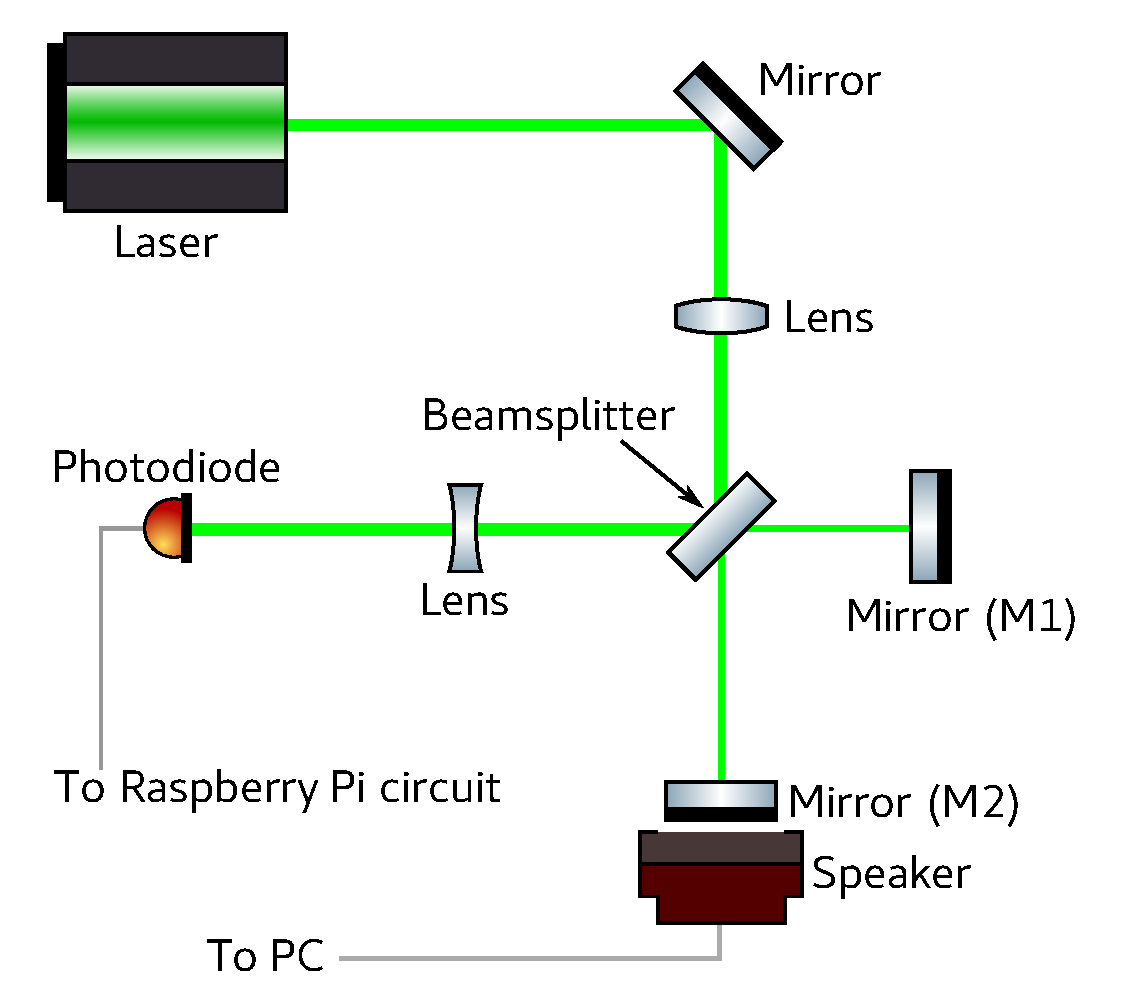
\includegraphics[width=0.49\textwidth]{figures/ifo_schematic_photodiode_edit.pdf}
	\caption{
Michelson interferometer schematic. 
The schematic is identical to Figure~\ref{fig:interference_pattern} except that the data is now recorded using a photodiode and Raspberry Pi instead of a webcam. 
}
	\label{fig:ifo_schematic_podo}
\end{figure}

\begin{figure*}
	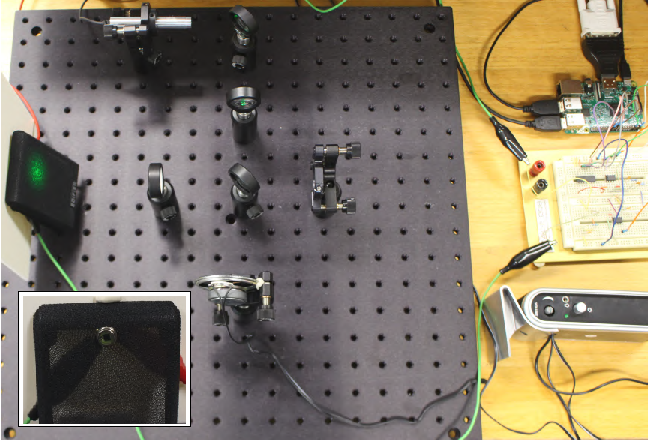
\includegraphics[width=.6\textwidth]{figures/setup_pic2.pdf}
\caption{Photograph of the optical microphone. The Michelson interferometer is shown on the left and the circuit and Raspberry Pi on the right. The interferometer is laid out as in Figure~\ref{fig:ifo_schematic_podo}. In the main image, the photodiode is placed behind the cloth screen. The inset shows a face-on view of the photodiode with the covering screen removed. See Appendix~\ref{app:circuit_diagram} for a circuit diagram and detailed photograph of the circuit.}
	\label{fig:setup_pic2}
\end{figure*}


\subsection{Anti-aliased output}
\label{sec:initialResultsOpMic}
% breakdown of all the filters used along the way
The optical microphone was tested on recordings of varying speech from different people and on music ranging from simple melodies and rhythms to full songs. 
The source audio was played through the speaker with the optical microphone recording for the full duration of the audio (around a minute long for most sources). When processing the results, we often only looked at the first ten seconds of each observation for efficiency.
During recordings, care was taken to ensure minimal activity around the interferometer to reduce environmental noise. 
The timeseries was then directly converted to a .wav file and played as an audio recording using the \textbf{io.wavfile.write} function from the Scipy~\cite{scipy} package in Python~\cite{python}, as before.

We find that the raw output of the optical microphone, collected without any further processing (except anti-aliasing), is noisy, with a loud bass hum throughout.
Each $10\,{\rm s}$ Fourier spectrum shows dominant AC mains noise with power ranging from the fundamental of the $50\,{\rm Hz}$ mains power up to and beyond its $8$th harmonic. \jam{[non-linear appendix, Andrew says to cite Feynman lectures on non-linear oscillations]}
We find that the mains power signal is present in data recorded without an injected audio signal as seen in the power spectral density in Figure~\ref{fig:psd_noise}.
The mains power is also present in data taken with the photodiode in complete darkness with a similar but weaker distribution as that shown in Figure~\ref{fig:psd_noise}).
The origin of the mains power signal is likely to be from the photodiode signal, or environmental noise from the rooms lighting and air conditioning, or a combination. 
Outside the mains noise, the power appears to peak broadly around 750 Hz, the origin or significance of which we don't know. 

\begin{figure}
	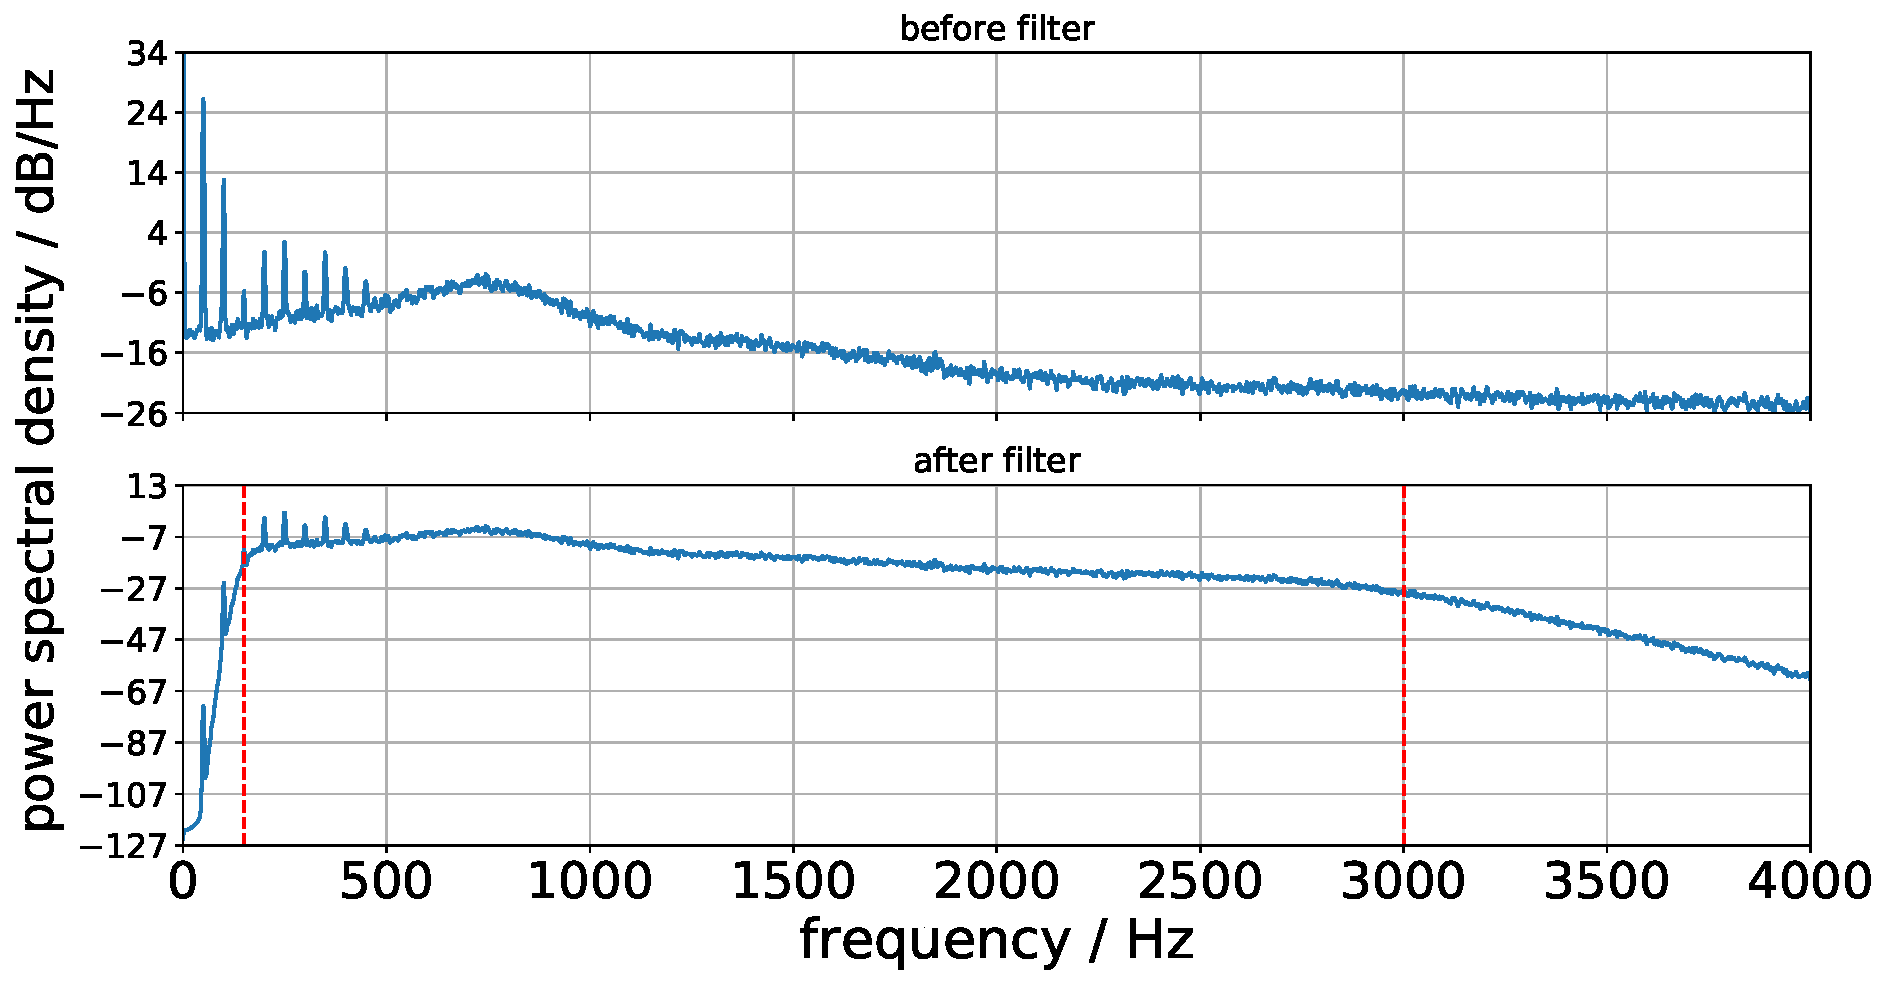
\includegraphics[width=.49\textwidth]{figures/psd_butterworth_14_6.pdf}
	\caption{\label{fig:psd_noise}
Power spectral density (PSD) of background noise (top) from the optical microphone (with the speaker off), and the PSD after applying a Butterworth bandpass filter (bottom) between the two frequencies marked with red, dashed lines. 
We see strong power from the $50\,{\rm Hz}$ mains hum and its harmonics (most likely from the photodiode circuit and the room’s lighting and cooling). Otherwise the PSD is fairly white. 
After filtering we see strong attenuation of all frequencies outside the band, but little change to the harmonics within the band.
}
\end{figure}


\subsection{Additional filters}
\label{sec:simple_filters}

Here we describe several approaches to remove the $50\,{\rm Hz}$ mains hum and its harmonics. 
We test these approaches on $1\,{\rm s}$ of data throughout this section as an illustrative example. 


\begin{figure*}
\begin{center}
% trim order is <left> <lower> <right> <upper>
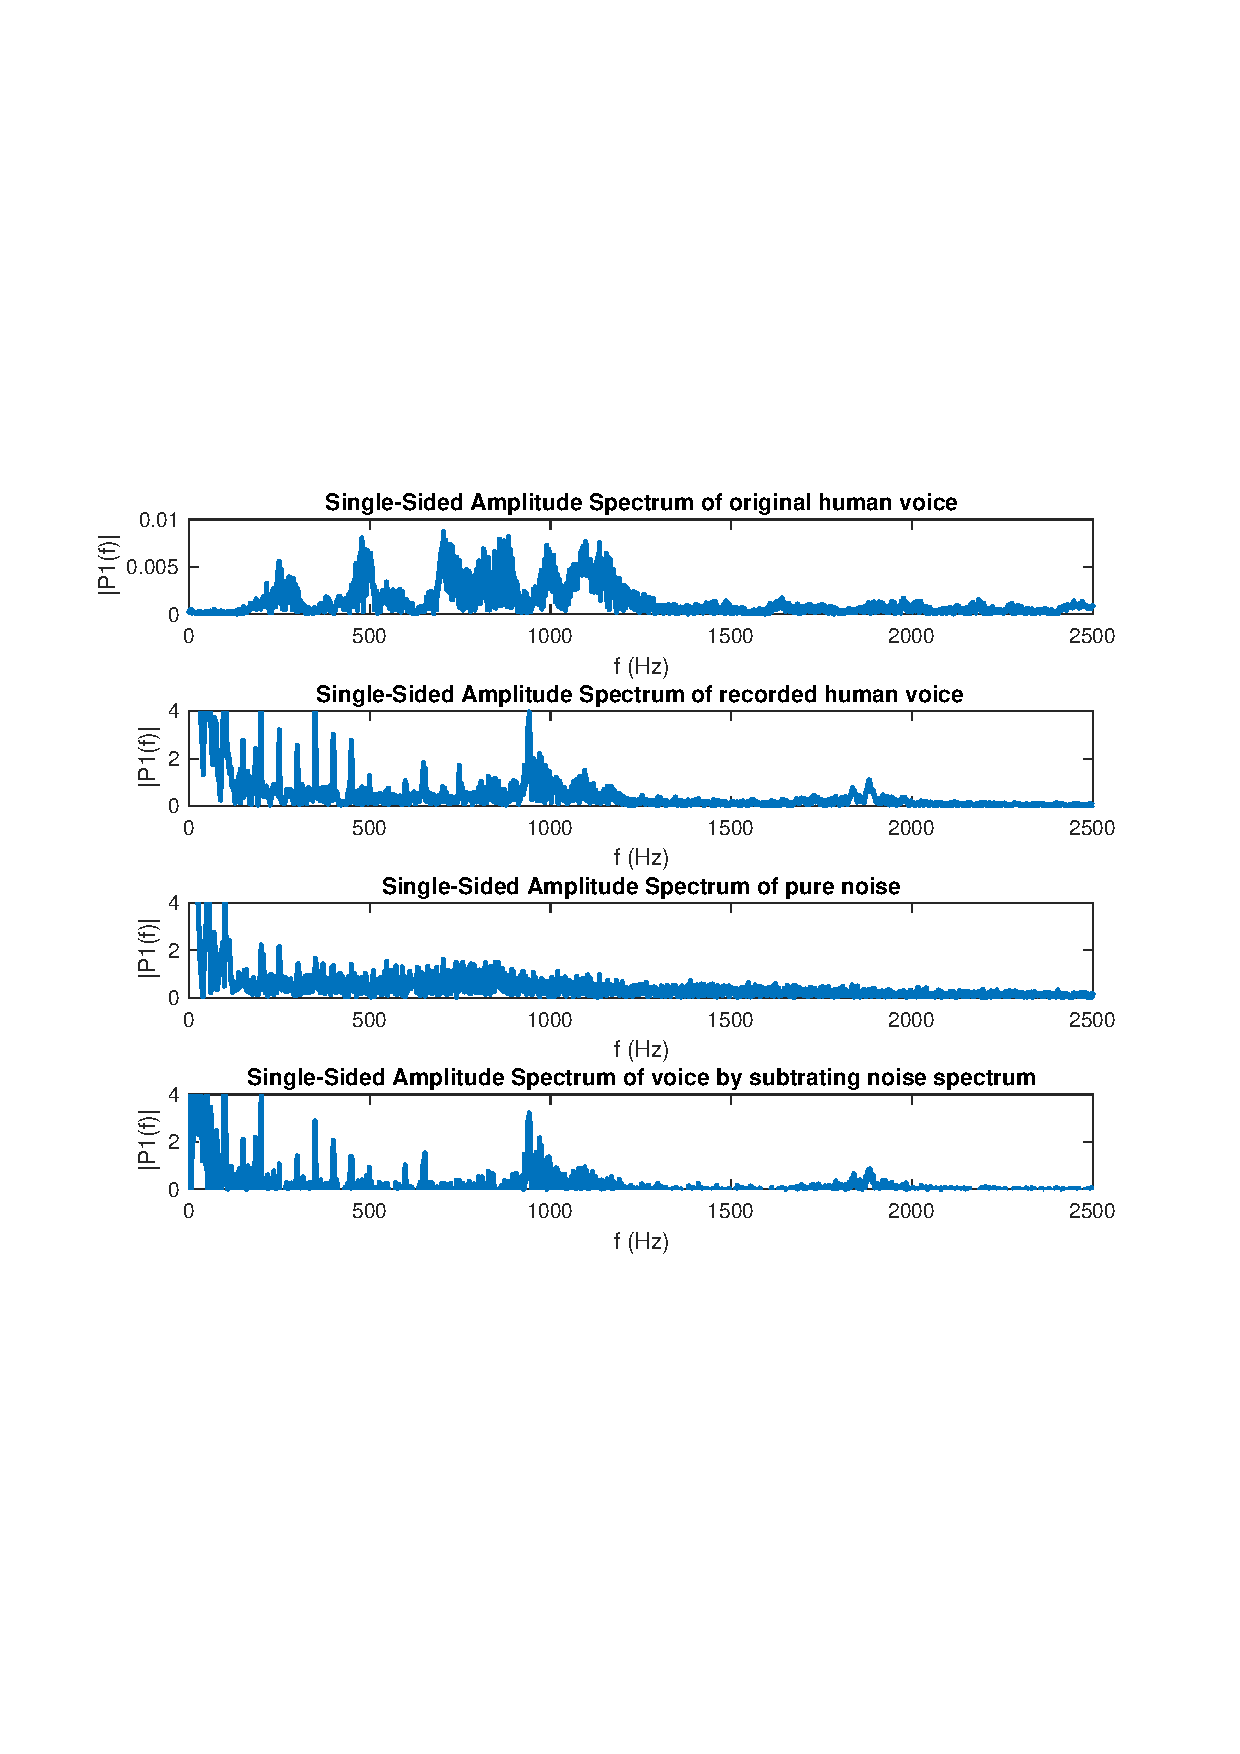
\includegraphics[width=\textwidth,trim={0cm 8.5cm 0 8cm},clip]{figures/freqSpectrumOriginalNoiseSubtracted.pdf}
\end{center}
\caption{\label{fig:noiseSubtract}
Frequency spectrum of a $1\,{\rm s}$ signal before the use of filters. 
The first panel shows the original frequency spectrum of the human voice recording (saying ``A cathode ...''). 
The second panel shows the spectrum recorded after the signal passes through the optical microphone (sampled at $16\,000\,{\rm Hz}$).
The third panel shows a noise-only recording from the optical microphone when no audio signal is being played. 
The fourth panel shows the result of subtracting the noise-only spectrum in the third panel from the recording in the second panel. 
We see no obvious improvement from this method. 
}
\end{figure*}

Fig.~\ref{fig:noiseSubtract} shows the frequency spectrum of $1\,{\rm s}$ of recorded speech. 
The first and second panels show the original signal before passing through the interferometer and the optical microphone recording of the signal respectively. 
An intuitive means to remove noise is to subtract the noise spectrum of the instrument directly from the signal spectrum. 
The third panel of Fig.~\ref{fig:noiseSubtract} shows a recording from the optical microphone with no audio signal. 
We see that the output noise is coloured, which reflects the non-linearity of the optical microphone.
The fourth panel of Fig.~\ref{fig:noiseSubtract} shows the frequency spectrum after the noise spectrum has been subtracted. 
We see no obvious improvement, which may be due to time-variant noise. 


The next step is to apply filters to the data. 
The ideal filter would be one that 
\begin{itemize}
\item[i)] completely attenuates the undesired parts of the spectrum, 
\item[ii)] does not change the rest of the spectrum, and 
\item[iii)] has smooth edges so as to not damage the signal after convolution. 
\end{itemize}
These three conditions are contradictory and any filter must compromise between them. 

We note that simply zeroing the frequency channel of each $50\,{\rm Hz}$ in the frequency spectrum is unsuccessful. 
Effectively, this multiplies the spectrum by a rectangular comb filter. 
It does remove the mains harmonics, however it audibly ruins the rest of the signal. 
Applying a filter in frequency space is equivalent to convolving the signal with the inverse Fourier transform of that filter. 
The inverse Fourier transform of a rectangular comb filter (a set of boxcars) is some combination of sinc functions, which significantly corrupt the signal. 

%A smoother comb filter significantly attenuates the spectrum between each harmonic so that the signal is no longer audible. 
% \jam{[re:comb filters. When I tried to comb filter it either was too sharp and so jumbled the whole signal in convolution. Or if smooth attenuated the signal away into noise. At least, that's what I remember. Changrong has a comb filter section anyway so I am happy dropping my unsuccessful attempts.]}

Applying a high-pass filter with cut-off frequency $150\,{\rm Hz}$ to the signal works well at removing the $50\,{\rm Hz}$ and $100\,{\rm Hz}$ harmonics.
However, mains harmonics above $100\,{\rm Hz}$ remain. 
The region above $100\,{\rm Hz}$ carries a lot of the fundamental frequencies of speech and music~\cite{speech_intelligibility}. 
Therefore, although a high-pass filter with a higher cut-off removes more harmonics, the played-back signal is unrecognisable. 
Applying a high-pass filter to the logarithm of the signal spectrum does not significantly improve on the above simple high-pass filter.

%We also tried applying a high-pass filter to the logarithm of the signal spectrum and then exponentiating back, but this didn’t significantly improve on the above simple high-pass


\begin{figure}
	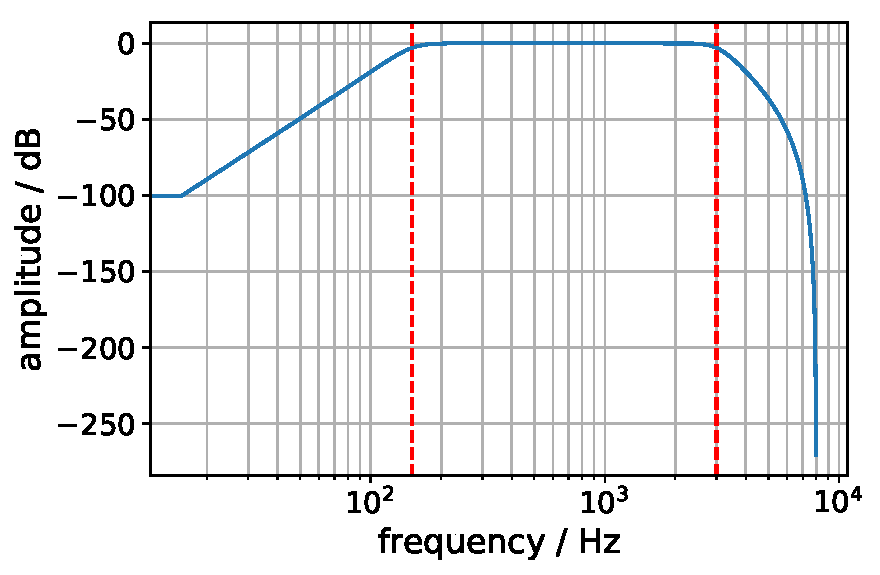
\includegraphics[width=0.49\textwidth]{figures/butterworth_150_3000.pdf}
	\caption{Butterworth bandpass filter frequency response, any amplitude beyond $-3\,{\rm dB}$ is significant attenuation (half power). The red, dashed vertical lines show the band limits of $150\,{\rm Hz}$ and $3\,{\rm kHz}$. Note the flat response within the band.}
	\label{fig:butterworth}
\end{figure}


Band-passing the signal similarly does not address the remaining harmonics above $100\,{\rm Hz}$. 
However, it does suppress other noise at higher frequencies. 
The best performing band-pass filter we find is a fifth order ($n = 5$) Butterworth filter over the range $150\,{\rm Hz}$--$3\,{\rm kHz}$ (beyond $2\,{\rm kHz}$ speech information content drops significantly~\cite{speech_intelligibility}). 
For a low-pass Butterworth filter with cut-off frequency $\omega_c$ and gain $\varepsilon$, the frequency response (attenuation at each frequency) as a function of frequency $\omega$ is:
\begin{equation}
\label{eq:butterworth}
H(\omega) = \left(1+\varepsilon^2 \left( \frac{\omega}{\omega_c} \right)^{2n}\right)^{-\frac{1}{2}}
\end{equation}

\jam{[Andrew wanted a quantitative comment about what the Butterworth does to the PSD, what do I use?]}
To construct a Butterworth band-pass filter, the low-pass filter in Eq.~\ref{eq:butterworth} is combined with a high-pass filter of similar form. 
The response of the filter used is shown in Figure~\ref{fig:butterworth}. 
The Butterworth filter performs the well as it is optimised to be `maximally flat' within the band region (prioritising condition (ii) above).
This filter improves on the above simpler filters but recordings of speech still have low intelligibility.
They can be recognised as speech without being understood.
Looking forward to Sec.~\ref{sec:logmmse}, results for the Butterworth filter are shown in combination with a speech enhancement technique. 

\begin{figure*}
\begin{center}
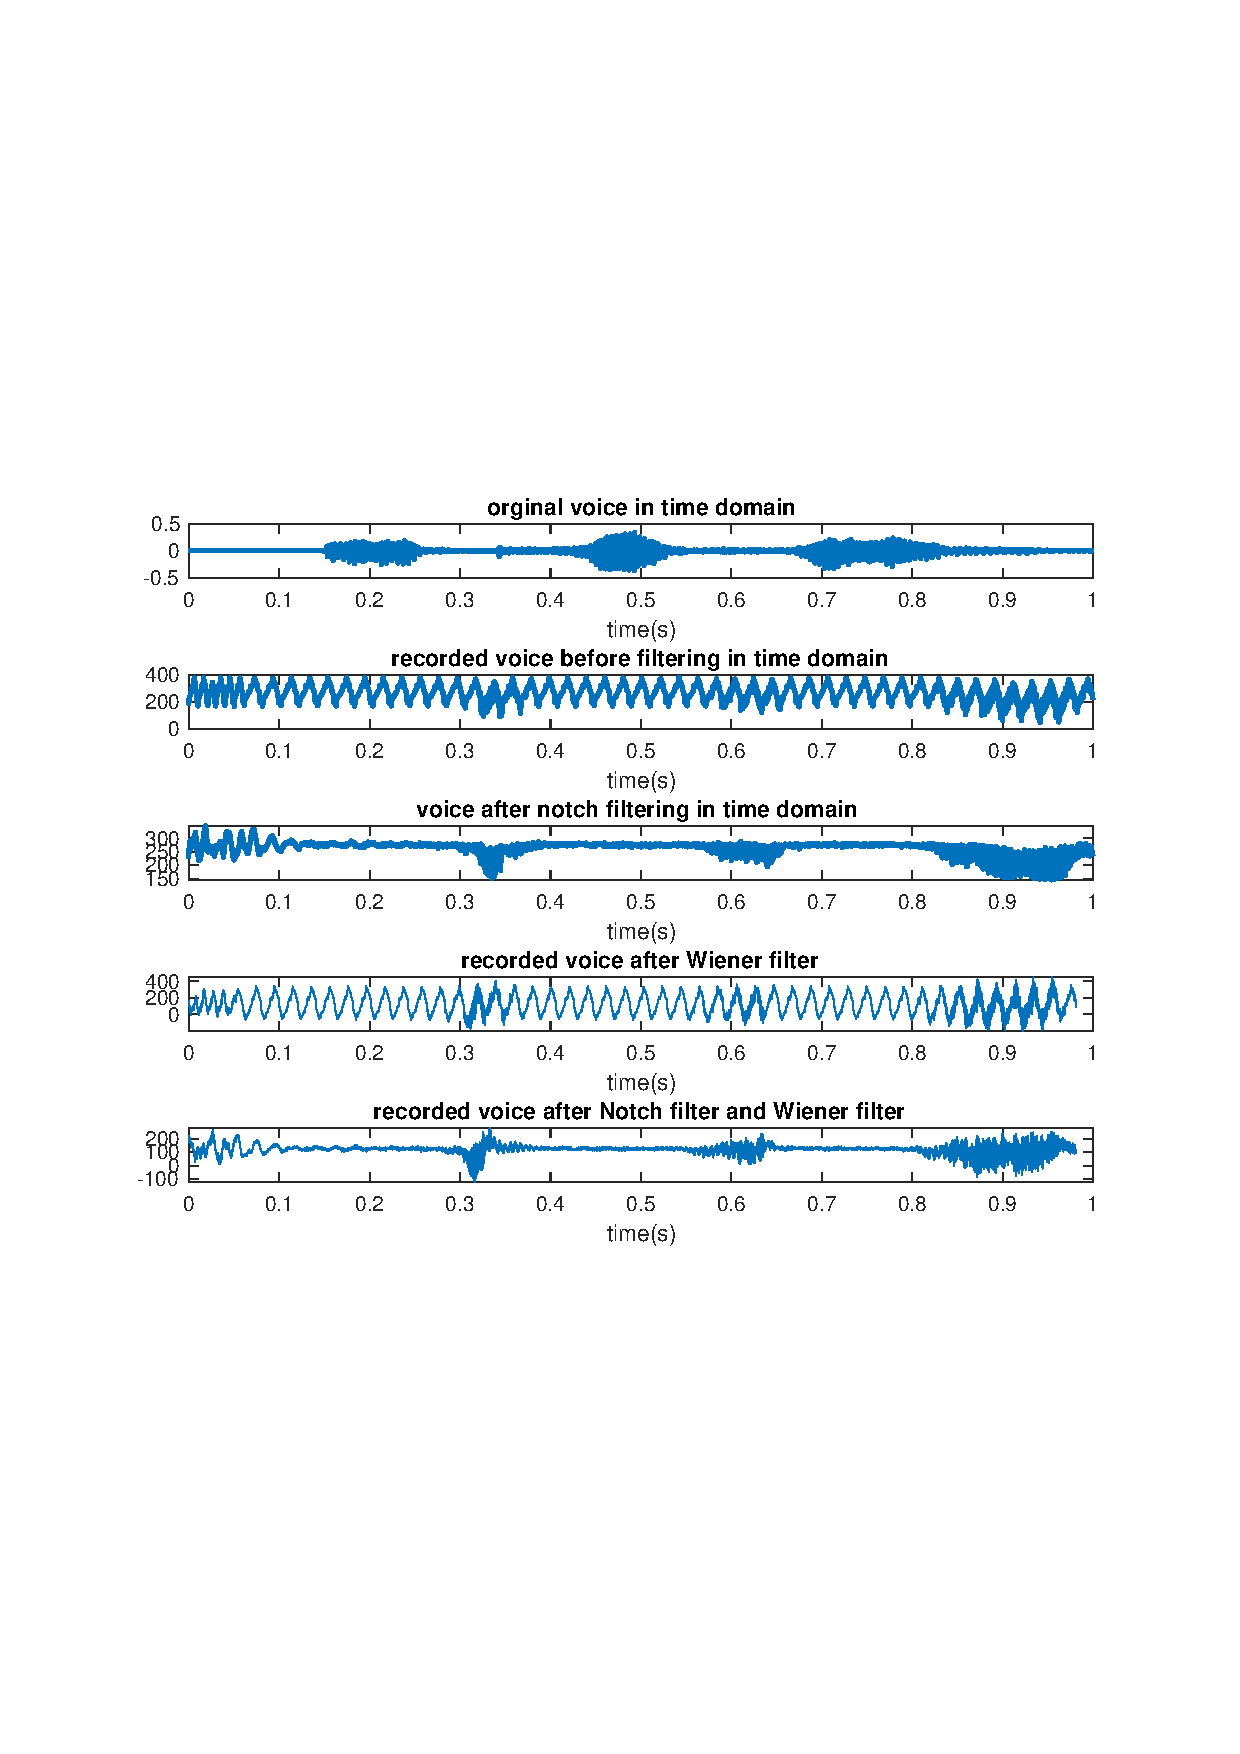
\includegraphics[width=\textwidth,trim={0cm 8.7cm 0 8.3cm},clip]{figures/timeSeriesNotchWiener.pdf}
\end{center}
\caption{\label{fig:timeNotchWiener}
Timeseries results for the notch and Wiener filters. 
The first panel shows the original speech recording which was played from the speaker. 
The second panel shows the data from the optical microphone before any filters are applied. 
The third and fourth panels show results after applying the notch and Wiener filter respectively. 
Finally, the fifth panel shows the result of applying both the notch and Wiener filter. 
}
\end{figure*}


\begin{figure*}
\begin{center}
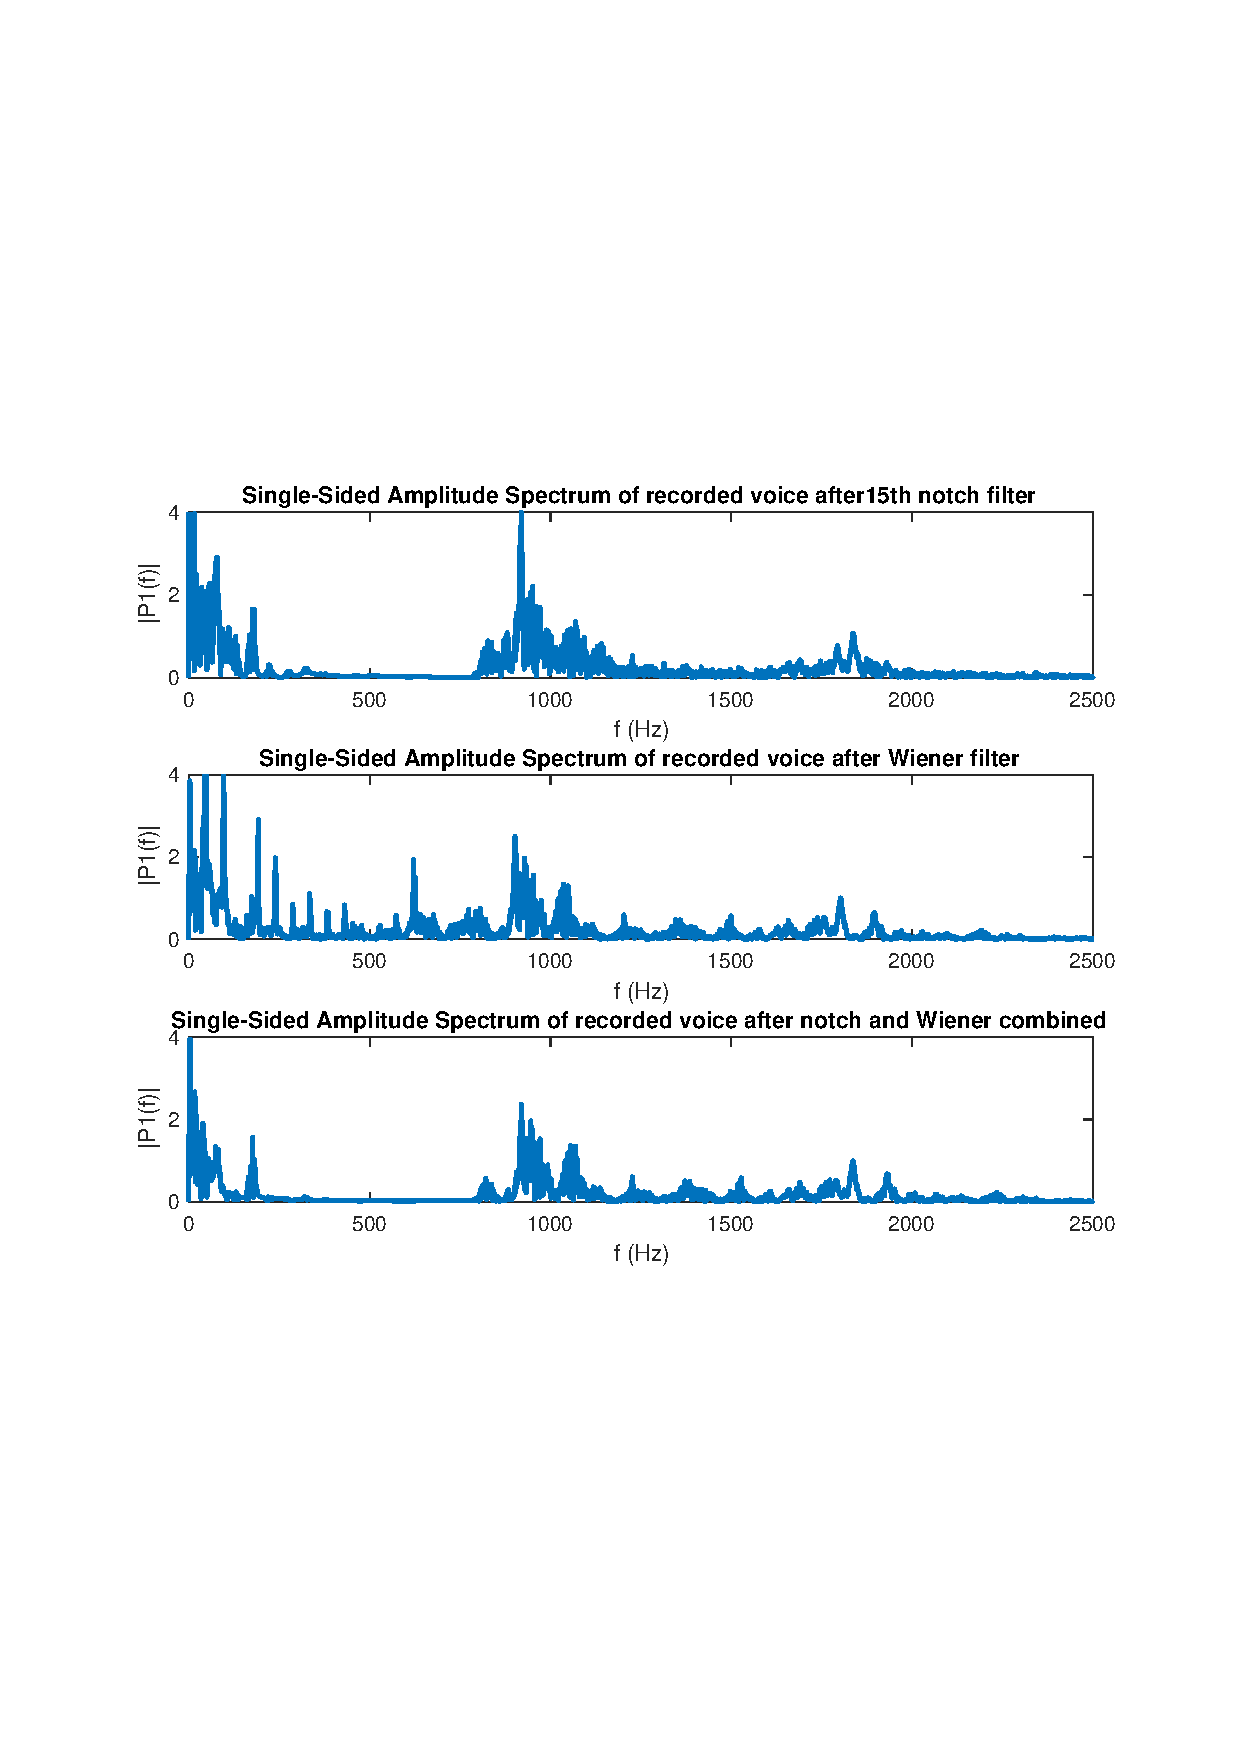
\includegraphics[width=\textwidth,trim={0cm 8.2cm 0 8cm},clip]{figures/freqNotchWiener.pdf}
\end{center}
\caption{\label{fig:freqNotchWiener}
Frequency spectrum results for the notch and Wiener filters. 
The first and second panels show the results of applying the notch and Wiener filter respectively.
The third panel shows the spectrum after applying both the notch and Wiener filters. 
The first, second, and third panels show the spectrum of the timeseries show in the third, fourth, and fifth panels of Fig.~\ref{fig:timeNotchWiener} respectively. 
}
\end{figure*}

We also consider a combined notch filter and Wiener filter.
Timeseries and frequency spectrum results are shown in Figs.~\ref{fig:timeNotchWiener} and ~\ref{fig:freqNotchWiener} respectively. 
The original signal is identical to that shown in Fig.~\ref{fig:noiseSubtract}.
The first and second panels of Fig.~\ref{fig:timeNotchWiener} show the original audio signal and the recording after passing through the optical microphone (i.e. the timeseries of the data shown in the first two panels of Fig.~\ref{fig:noiseSubtract}). 



\subsubsection{Cascade notched filter}
A straightforward method for removing hum noise and its harmonics is to use a sequence of notch filters centered at each of the frequency bins we want to remove. 
A typical transfer function of infinite impulse response (IIR) notch filter can be written as \citep{10.5555/541204}
\begin{equation}
    \label{eqn:notch}
    H(z)=\frac{1+\alpha}{2}\frac{1-2\beta z^{-1}+z^{-2}}{1-\beta(1+\alpha)z^{-1}+\alpha z^{-2}}
\end{equation}
where $\alpha$ and $\beta$ are self-tuned parameters which adjust the locations of poles and zeros. 
By allowing the numerator and demoninator of $H(z)$ to be zero, we can find the corresponding locations of zeros and poles of the filter. 
Notice zeros are at $e^{\pm jw_0}, \text{where } w_0=\cos^{-1}(\beta)$, and poles are at $re^{\pm j\phi}, \text{where } r=\sqrt{\alpha},\phi=\cos^{-1}(\beta(1+\alpha)/(2\sqrt{\alpha}))$.
At $w_0$, the magnitude response will be zero. 
Thus, we can calculate $\beta$ setting $w_0$ to be the frequency we want to remove. 
The parameter $\alpha$ affects the bandwidth ($B_w$) of the filter and has the relation $B_w=\cos^{-1}(\frac{2\alpha}{1+\alpha^2})$. \\
In our paper, we first decide $\beta$ for each filter. 
We locate hum noise spectrum at around $50k\,{\rm Hz}$ where the integer $k=1,2,\dots,15$. 
For each $k$, we build a notch filter to filter out the specific frequency bin approximately at $50k \, {\rm Hz}$. 
We then alter the parameter $\alpha$ to determine the bandwidth of each filter. 
On one side, the bandwidth should be as narrow as possible to avoid disturbing useful signals. 
This can be achieved through increasing orders of the filter (add more poles and zeros). 
On the other side, the bandwidth should have enough residues to account for the uncertainty of our pinpointing the location of hum noise. 
After considering these two aspects, we are now able to get the ideal transfer function for each filter. 
The whole cascaded filter is achieved by multiplying them together, 
\begin{equation}
    \label{eqn:notch15}
    H(z)=H_1(z)H_2(z)\dots H_k(z),k=1,2,\dots 15\,,
\end{equation}
where $H(z)$ denotes the transfer function of the full cascaded notch filter, and $H_k(z)$ denotes one single notch filter for removing $50k \, {\rm Hz}$ frequency. 
We use the built-in MATLAB filter design toolbox to help us realize a well performed cascaded notch filter (each filter has order 6).  
The magnitude response of the first five notch filters are shown in Fig.~\ref{fig:notchMagResponse}. 
\begin{figure}
\begin{center}
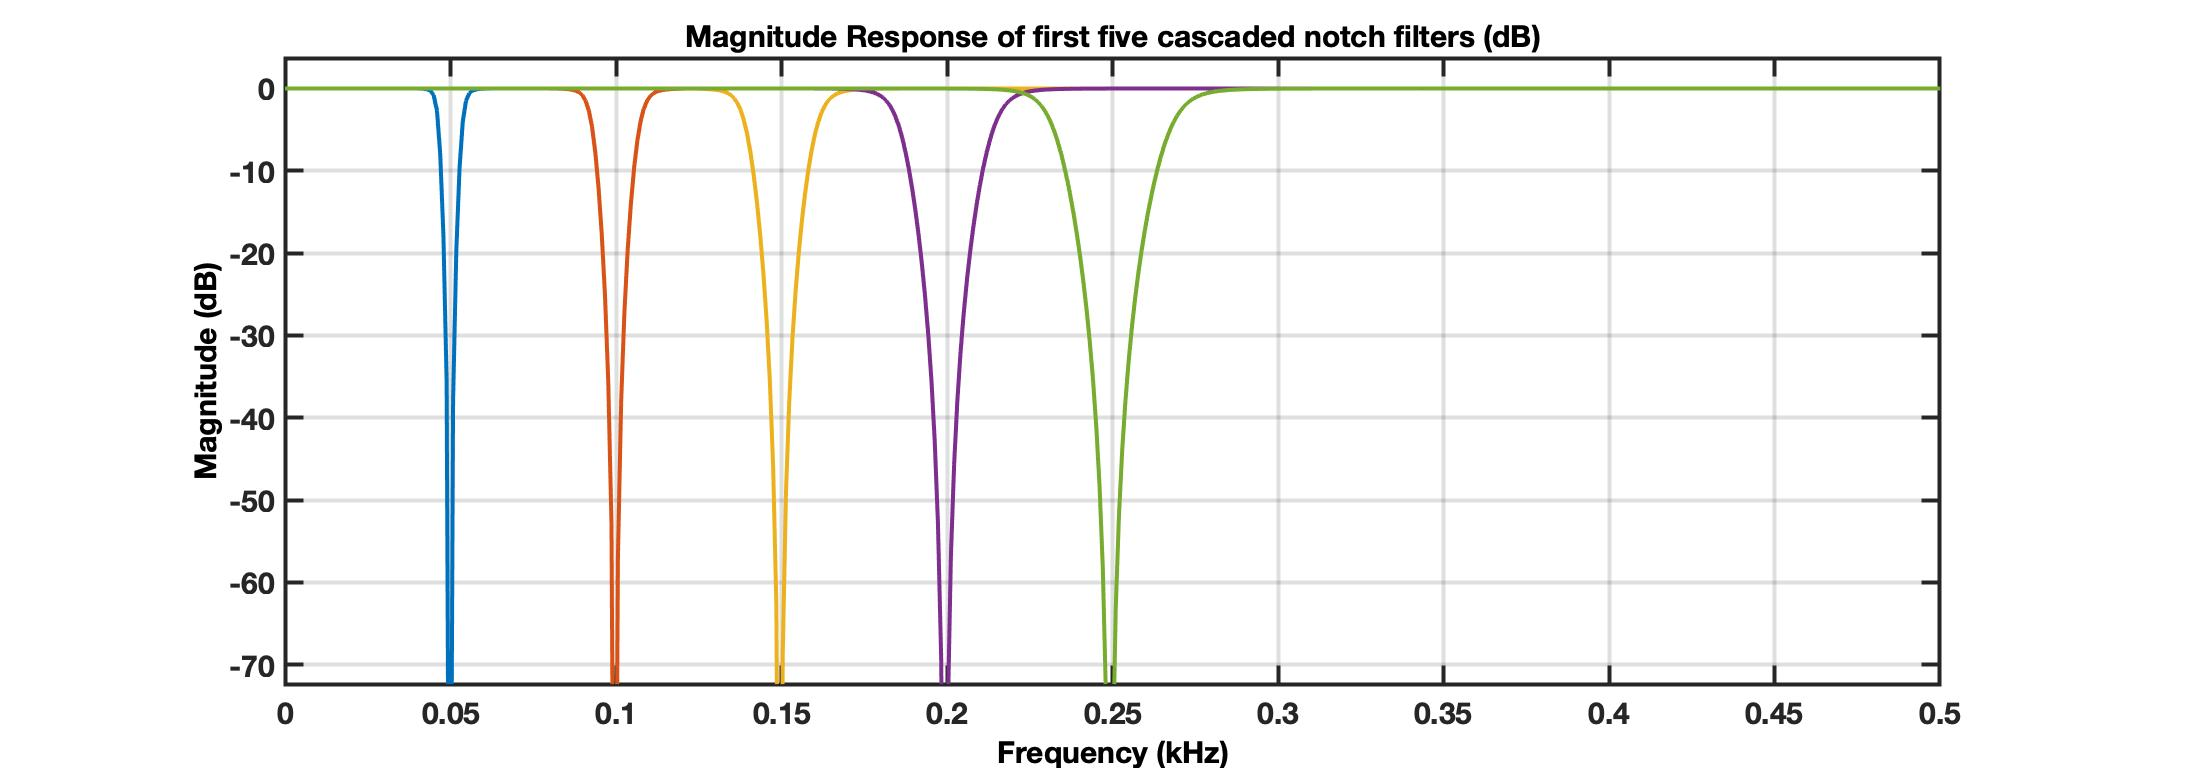
\includegraphics[width=.49\textwidth]{figures/1111}
\end{center}
\caption{\label{fig:notchMagResponse}
Magnitude response for the first five notches of the $15$ cascaded notch filter described by Eqns.~\ref{eqn:notch} and ~\ref{eqn:notch15}. 
}
\end{figure}


The timeseries and frequency spectrum results of the notch filter are shown in the third panel of Fig.~\ref{fig:timeNotchWiener} and the first panel of Fig.~\ref{fig:freqNotchWiener}. 
We seen that the mains harmonics are significantly attenuated in comparison to the analysis in Fig.~\ref{fig:noiseSubtract}. 

%A notch filter attenuates signals in specific frequency bands. 
%We apply a $15$ cascaded notched filter to remove the mains noise and its harmonics up to $750\,{\rm Hz}$. 
%\han{should we include here a mathematical description of the $15$ cascade notch filter?}
%\jam{[Yes, I have no idea what a cascaded notched filter is and I'm an author!]}



\subsubsection{Weiner Filter}

We use vector $\textbf{x}=\{x(0),\dots x(N-1)\}$ to denote the noisy speech signal sequence. Assume original clean signal is $\textbf{s}=\{s(0),\dots,s(N-1)\}$, and the noise sequence $\textbf{w}=\{w(0),\dots,w(N-1)\}$. We then have
\begin{equation}
    \textbf{x}=\textbf{s}+\textbf{w}
\end{equation}
Based on the observation data$\textbf{x}$, our goal is to estimate s, such that the error between $\textbf{x}$ and estimated $\mathit{\hat{s}}$ is minimized in the mean square sense, we write
\begin{equation}
    \hat{\textbf{s}}=\mathop{\arg\min}_{\textbf{s}}||\textbf{x}-\textbf{s}||_2^2
\end{equation}
Under the assumptions that observed data is wide sense stationary and noise sequence is stationary, uncorrelated with signal, we represent the $n$th order Wiener filter by its coefficients $\textbf{h}=\{h(0),\dots(n)\}$. 
The famous Wiener-Hopf equation \citep{noble1959methods} provides us a way to determine $\textbf{h}$, which can be expressed as 
\begin{equation}
\label{winer-hopf}
\begin{bmatrix}  
r_{xx}[0]&r_{xx}[1]&\dots& r_{xx}[n]\\
r_{xx}[1]&r_{xx}[0]&\dots &r_{xx}[n-1]\\
\vdots&\vdots&\ddots&\vdots\\
r_{xx}[n]&r_{xx}[n-1]&\dots &r_{xx}[0]
\end{bmatrix}
\begin{bmatrix}
h[0]\\
h[1]\\
\vdots\\
h[n]
\end{bmatrix}=
\begin{bmatrix}
r_{ss}[0]\\
r_{ss}[1]\\
\vdots\\
r_{ss}[n]
\end{bmatrix}
\end{equation}

\begin{equation*}
\left\{
\begin{array}
r_{xx}[n]=E[x[i]x[i+n]] \\ 
r_{ss}[n]=E[s[i]s[i+n]]
\end{array} \right\}  
\end{equation*}
where $r_{xx}$ and $r_{ss}$ is the auto-correlation function of $x$ and $s$.
If further, we do not need to guarantee the causality of Wiener filter, in other words, we estimate current signal based on both past and future observations, Eq. \ref{winer-hopf} can then be represented in the frequency domain, which is
\begin{equation}
\label{wiener}
    H(f)=\frac{P_{ss}(f)}{P_{xx}(f)}=\frac{P_{ss}(f)}{P_{ss}(f)+P_{ww}(f)}
\end{equation}
where $P_{xx}(f),P_{ss}(f),P_{ww}(f)$ stands for the frequency spectrum of noisy observations, clean signal and pure noise respectively. Intuitively, from Eq. \ref{wiener}, we can see Wiener filter amplifies input signal where signal to noise ratio (SNR) is high, and weaken the signal where SNR is low.
Notice that since this filter is non-causal, which may not be suitable for real time signal processing. More detailed analysis can be found in \citep{10.5555/151045}. In our case, we construct a causal Wiener filter based on Eq. \ref{winer-hopf}, and set the length of the filter to be 100. Large n smooths the input signal further, while cause more delay and requires more memory meanwhile. $n=100$ is a relatively reasonable choice for balancing these effects.

%The Wiener filter produces an estimated signal $\hat{x}$ using linear time-invariant filtering. 
%It minimizes the mean square error $\mathbb{E}[(\hat{x}-x)^2]$ between $\hat{x}$ and the actual signal $x$~\citep{verhoeven2009robust}.
%\han{should we add more details here too?} \jam{[seconded]}
%The timeseries and frequency spectrum results of the Wiener filter are shown in the fourth panel of Fig.~\ref{fig:timeNotchWiener} and the second panel of Fig.~\ref{fig:freqNotchWiener} respectively. 
%The timeseries is visibly cleaner, however there is a strong noise hum. 


\subsubsection{Combined Notch and Weiner filter}
The Wiener filter makes use of statistical information from the speech data and noise. 
It amplifies the part of the signal with high SNR, while suppressing the part with low SNR. 
It is implemented in the form of a finite response filter, which ensures linear phase response and stability at the cost of high orders. 
By comparison, the notch filter is based on directly removing the unwanted frequency components. 
It is implemented in the form of an infinite impulse response fileter. 
Although it significantly decreases the order of the filter, it unavoidably introduces nonlinear phase and instability. 

Combining the notch and Wiener filter, we have a trade off between the two filters, which shows better performance in filtering out different noise components (white noise plus hum noise). 
The results from the combination of notch and Wiener filters are visibly cleaner as shown in the final panels of Figs.~\ref{fig:timeNotchWiener} and ~\ref{fig:freqNotchWiener} for the timeseries and spectrum respectively 



%The combination of the notch filter and the Wiener filter produces a cleaner signal than either individually. 
%The time series and spectrum results are shown in the final panels of Figs.~\ref{fig:timeNotchWiener} and ~\ref{fig:freqNotchWiener} respectively.

%The ideal filter would be one that i) completely attenuates the undesired parts of the spectrum, ii) does not change the rest of the spectrum, and iii) has smooth edges so as to not damage the signal after convolution. 
%These three conditions are contradictory and any filter must compromise between them. 
%The above simple filters fail one or more of i)--iii). 
%The Butterworth filter performs the best as it is optimised to be `maximally flat' within the band region, prioritising the second condition.
%\han{see note from Andrew and ask James about this}






%\han{Is it worth also including some plots to show how the different filters perform? E.g. a PSD with comb filter, high pass filter, Butterworth filter?}

% Note that we also replicated the Viterbi algorithm results from before with the photodiode, but only with the mains hum removed and high-passing above 100Hz, else the algorithm never selected the signal. Except for being over audible frequencies, there isn’t much difference in the tracking once these filters are applied.


\subsection{logMMSE estimator}
\label{sec:logmmse}
% logMMSE

Speech enhancement for a noisy channel is a classic problem in signal processing. 
Hu~\&~Loizou~(2006)~\cite{SubjectiveComparison} compare 13 speech enhancement methods and find the best to be a log minimum mean-square error (log-MMSE) estimator. 
This type of estimator is based on work by Ephraim~\&~Malah~(1984)~\cite{Ephraim1984SpeechEU_logMMSE} into speech enhancement by minimising the mean square error (MSE) to the logarithm of the spectral (Fourier) amplitude.
The logarithm approximates the response of the human ear~\cite{SubjectiveComparison}.


In this work we use an existing implementation~\cite{logmmse} of the logMMSE estimator. 
Applying this estimator to the optical microphone output produced dramatically cleaner results. 

In Figures~\ref{fig:logMMSE_timeseries} and~\ref{fig:logMMSE_spectrum} we present results from playing a speech recording through the optical microphone. 
Figure~\ref{fig:logMMSE_timeseries} shows the anti-aliased photodiode time series from before (top panel) and after (bottom panel) applying the logMMSE filter. 
Figure~\ref{fig:logMMSE_spectrum} shows the corresponding spectra before (top panel) and after (bottom panel) the logMMSE filter. 
Comparing the before and after spectra shows significant attenuation of all mains harmonics as well as a general smoothing of the spectrum. 

\begin{figure*}
	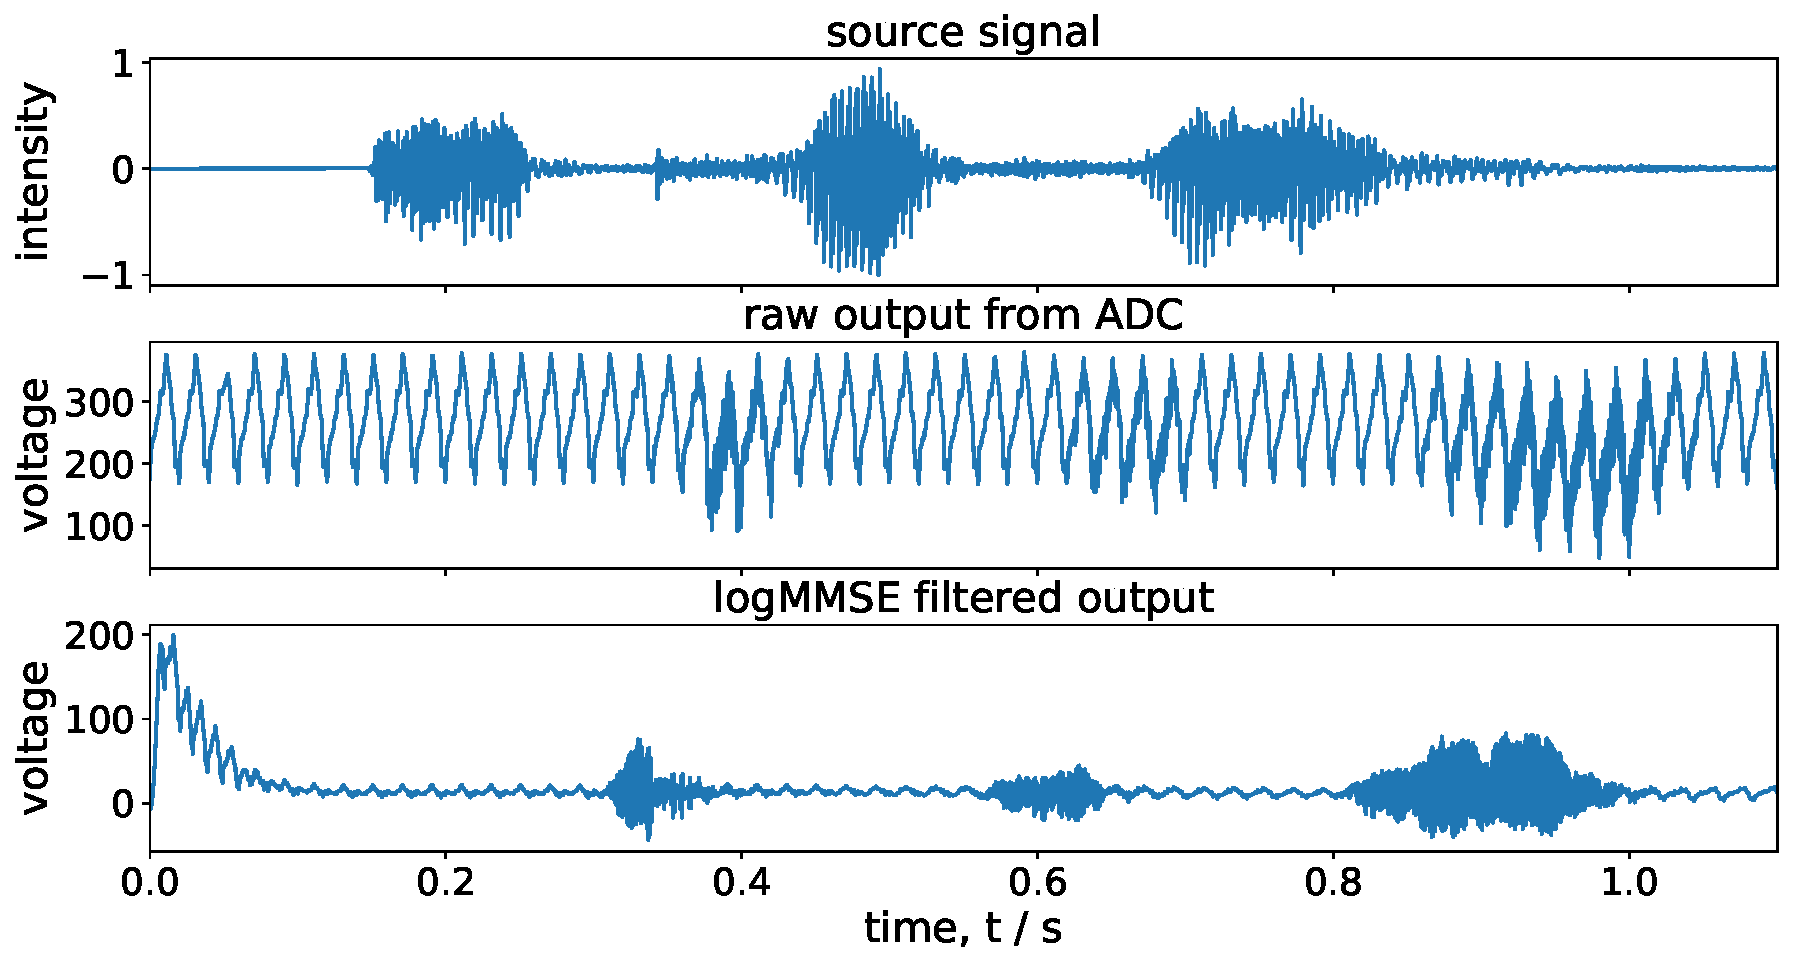
\includegraphics[width=\textwidth]{figures/combined_timeseries_melatos.pdf}
	\caption{Time series of an adult male voice (saying ``A cathode ...'') showing the source (top panel), the optical microphone recording (middle panel), and the recording after filtering with the logMMSE estimator (bottom panel). One second of the one minute recording is shown. The rise at the start of the bottom panel is expected when filtering a signal of finite duration.}
	\label{fig:logMMSE_timeseries}
\end{figure*}

\begin{figure*}
	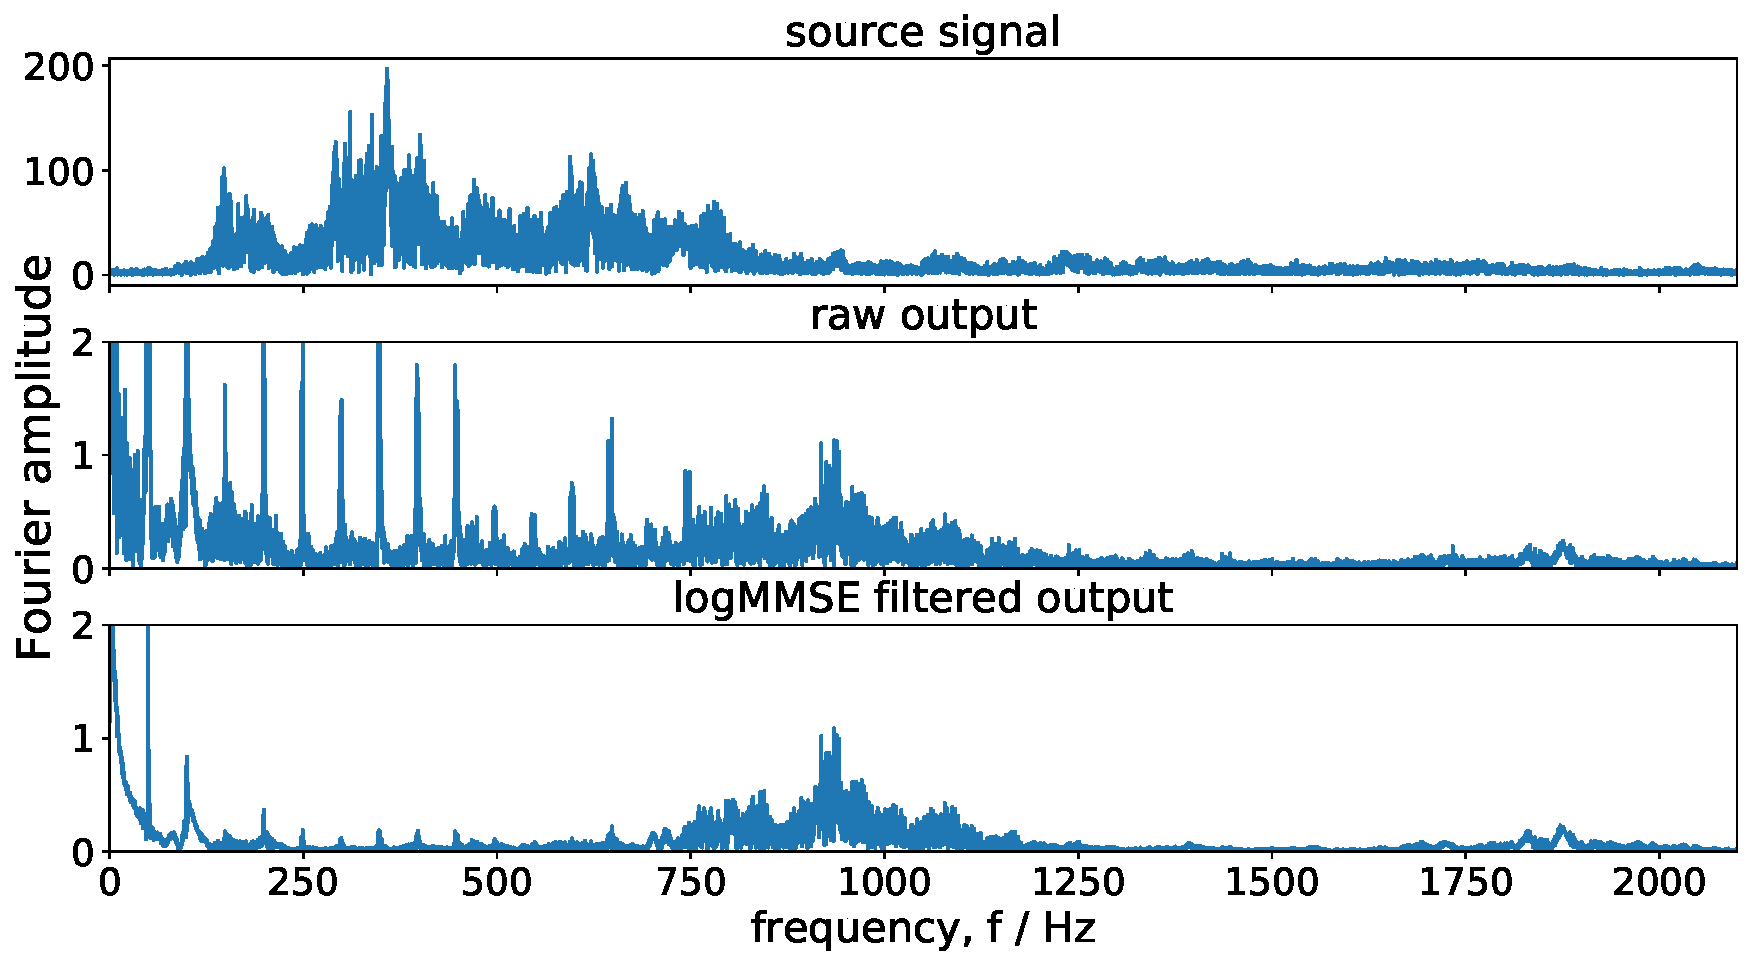
\includegraphics[width=\textwidth]{figures/combined_spectrum_melatos.pdf}
	\caption{Spectrum of optical microphone recording of the same adult male voice in Fig.~\ref{fig:logMMSE_timeseries} showing the source (top panel), the optical microphone recording (middle panel), and the recording after filtering with the logMMSE estimator (bottom panel). The spectrum shows only a detail of the total frequency domain (there is little activity at higher frequencies) and has truncated peaks at amplitude 2 which otherwise dominate the plot.}
	\label{fig:logMMSE_spectrum}
\end{figure*}


We also find improvement with music recordings.
After applying the estimator, simple chords and drums can be heard clearly. 
However more complex melodies are sometimes completely absent. 
From observation, this is especially true for instruments of certain timbres (harmonic profiles), in particular flutes and violins.
This could be a perceptual effect or a frequency dependence somewhere in the optical microphone. 
Speculating, perhaps the speaker-mirror oscillates more at at low frequencies and so instruments like electric bass and drums are louder in the results.


Overall, we find that the intelligibility of speech remains low. 
The played-back voice sounds mumbled and indistinct. 
The estimator removes most of the background noise, but does not clarify the speech. 
To address these problems with the recordings we need to determine whether the signals that are audibly missing (the diction in the speech and complex melodies in music) are indeed being transmitted through the optical microphone at all. 
This requires a better understanding of the system.
% The fringe counting problem of the detector, wherein multiple fringes passing over the array in a single speaker deflection artificially raises the frequency, was noticeable in the speech recordings when compared to the source audio. However, upon comparing injected pure tones, the increase appears to be minimal and inconsistent, at around 5Hz maximum difference. An simple explanation is that the speaker deflections are small compared to manual pressing on the optical table.



\end{document}
